\documentclass[10pt]{beamer}

\usepackage[T2A]{fontenc}
\usepackage[utf8]{inputenc}
\usepackage[russian,english]{babel}

\usefonttheme[onlymath]{serif}

\usetheme[progressbar=frametitle]{metropolis}
\usepackage{appendixnumberbeamer}

\usepackage{booktabs}
\usepackage[scale=2]{ccicons}

\usepackage{pgfplots}
\usepgfplotslibrary{dateplot}

\usepackage{xspace}
\newcommand{\themename}{\textbf{\textsc{metropolis}}\xspace}
\newcommand{\TODO}[1]{\textbf{\textcolor{red}{TODO: #1}}}

\date{}
\author{Екатерина Тузова}


\title{Лекция 10}
\subtitle{Линейная регрессия}

\begin{document}	

\section{Разбор летучки}

\frame{\titlepage}

\begin{frame}\frametitle{Регрессия}
	$X$-- объекты в $\mathbb{R}^n$; Y — ответы в $\mathbb{R}$\\
	$X^l = (x_i, y_i)_{i=1}^l$ -- обучающая выборка\\
	$y_i = y(x_i)$, \qquad $y : X \rightarrow Y$ -- неизвестная зависимость\\
	\bigbreak
	\pause
	$a(x) = f (x, w)$ -- модель зависимости,\\
	$w \in \mathbb{R}^p$ -- вектор параметров модели.\\
	\bigbreak
\end{frame}

%\begin{frame}{Метод максимума правдоподобия}
%	Модель данных с некоррелированным гауссовским шумом:\\
%	$$y(x_i) = f (x_i, w) + \varepsilon_i, \hspace{5mm} \varepsilon_i \in N (0, \sigma_i^2), i = 1, \dots, l$$\\
%	\bigbreak
%	\pause
%	\alert{Вопрос}: Как выглядит плотность одномерного Гауссовского распределения?
%\end{frame}
%
%\begin{frame}{Нормальное распределение}
%	\begin{figure}[htbp]
%	  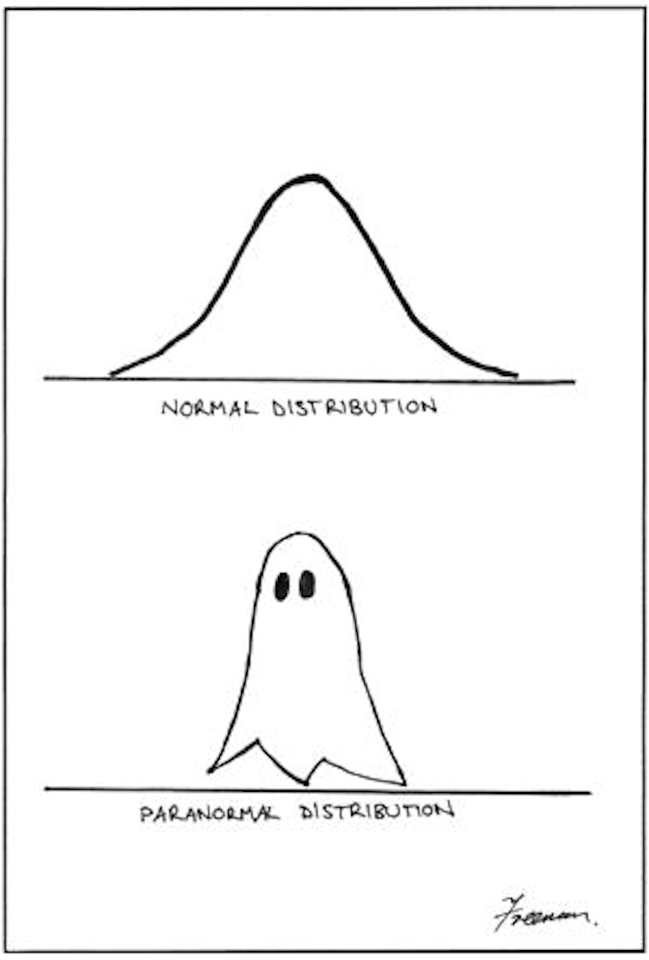
\includegraphics[height=200pt, keepaspectratio = true]{images/paranormal}   
%	\end{figure}
%\end{frame}
%
%\begin{frame}{Нормальное распределение}
%	\begin{figure}[htbp]
%	  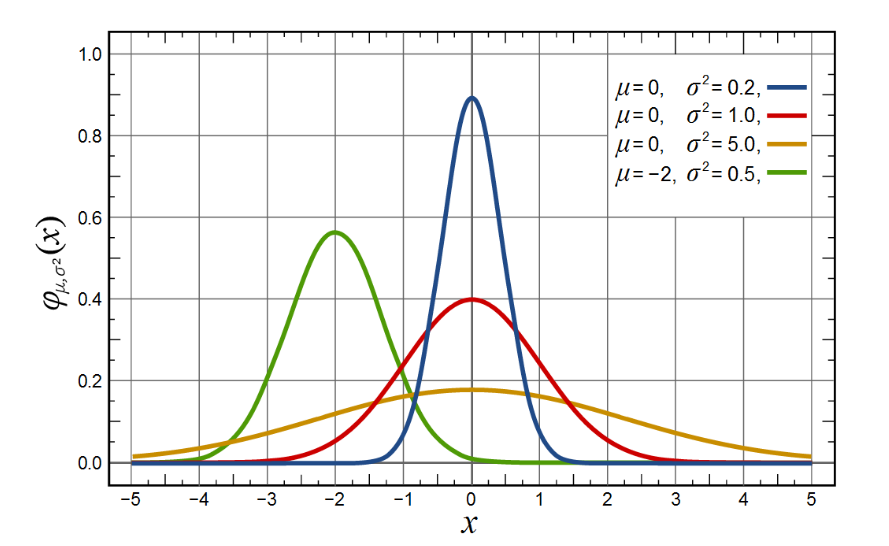
\includegraphics[height=200pt, keepaspectratio = true]{images/gauss}   
%	\end{figure}
%\end{frame}
%
%\begin{frame}{Метод максимума правдоподобия}
%	Метод максимума правдоподобия (ММП):\\
%	$$L(\varepsilon_1, \dots, \varepsilon_l | w) = \prod\limits_{i=1}^l p(\varepsilon_i) = \prod\limits_{i=1}^l \frac{1}{\sigma_i \sqrt{2\pi}} \exp (-\frac{\varepsilon_i^2}{2\sigma_i^2}  ) \rightarrow \max\limits_{w}$$\\
%	\pause
%	$$- \ln L(\varepsilon_1, \dots, \varepsilon_l| w) = const(w) + \frac{1}{2} \sum\limits_{i=1}^l \frac{(f(x_i, w) - y_i)^2}{\sigma_i^2}  \rightarrow \min\limits_{w}$$\\
%\end{frame}
%
%\begin{frame}{Метод максимума правдоподобия}
%	Метод максимума правдоподобия (ММП):\\
%	$$- \ln L(\varepsilon_1, \dots, \varepsilon_l| w) = const(w) + \frac{1}{2} \sum\limits_{i=1}^l \frac{(f(x_i, w) - y_i)^2}{\sigma_i^2}  \rightarrow \min\limits_{w}$$\\
%	\bigbreak
%	\pause
%	Метод наименьших квадратов: $$Q(w,X^l) = \sum\limits_{i=1}^l \alpha_i (f (x_i, w) - y_i)^2 \rightarrow \min\limits_{w}$$\\
%	\bigbreak
%	\pause
%	\alert{Удивительный факт}: Постановки МНК и ММП, совпадают, причём веса объектов
%	обратно пропорциональны дисперсии шума, $\alpha_i = \sigma_i^{-2}$
%\end{frame}

{\foot{Метод наименьших квадратов}
\begin{frame}{Многомерная линейная регрессия}
	$x^1, \dots, x^n$ -- числовые признаки\\
	Модель многомерной линейной регрессии:\\
	$$f (x, w) = \sum\limits_{j=1}^n w_j x^j, \qquad w \in \mathbb{R}$$\\
	\bigbreak
	\pause
	Функционал квадрата ошибки:\\
	$$Q(w,X^l) = \sum\limits_{i=1}^l (f (x_i, w) - y_i)^2  \rightarrow \min\limits_{w}$$\\
\end{frame}
}

\begin{frame}{Матричное представление}
	$$\underset{l \times n}{X} = \begin{pmatrix}
	  x_1^1 & \dots & x_1^n \\
	  \dots & \dots & \dots\\
	  x_l^1 & \dots & x_l^n
	 \end{pmatrix} \qquad 
	 \underset{l \times 1}{y} = \begin{pmatrix}
	  y_1 \\
	  \dots\\
	  y_l
	 \end{pmatrix} \qquad
	 \underset{n \times 1}{w} = \begin{pmatrix}
	  w_1 \\
	  \dots\\
	  w_n
	 \end{pmatrix}$$ \\
	\bigbreak
	\pause
	Функционал квадрата ошибки:\\
	$$Q(w,X^l) = \sum\limits_{i=1}^l (f (x_i, w) - y_i)^2  = \Vert Xw - y \Vert^2 \rightarrow \min\limits_{w}$$\\
\end{frame}

\begin{frame}{Нормальная система уравнений}
	Необходимое условие минимума:\\
	$$\frac{\partial Q(w)}{\partial w}  = 2 X^T(X w - y) = 0$$\\
	\pause
	\bigbreak
	Откуда следует нормальная система задачи МНК:\\
	$$X^T X w = X^T y$$\\
	$X^T X$ -- ковариационная матрица признаков $x^1, \dots, x^n$\\
\end{frame}

\begin{frame}{Нормальная система уравнений}
	Нормальная система задачи МНК:
	$$X^T X w = X^T y$$\\
	\pause
	Решение системы:\\
	$$w^* = (X^T X)^{-1} X^T y = X^{+} y$$\\
	$X^{+}$ -- псевдообратная матрица\\
	\bigbreak
	\pause
	Значение функционала: $Q(w^*) = \Vert P_X y - y \Vert^2$\\
	\bigbreak
	где $P_X = X X^{+} = X(X^T X)^{-1} X^T$ -- проекционная матрица
\end{frame}

\begin{frame}{Геометрический смысл}
	\begin{figure}[htbp]
	  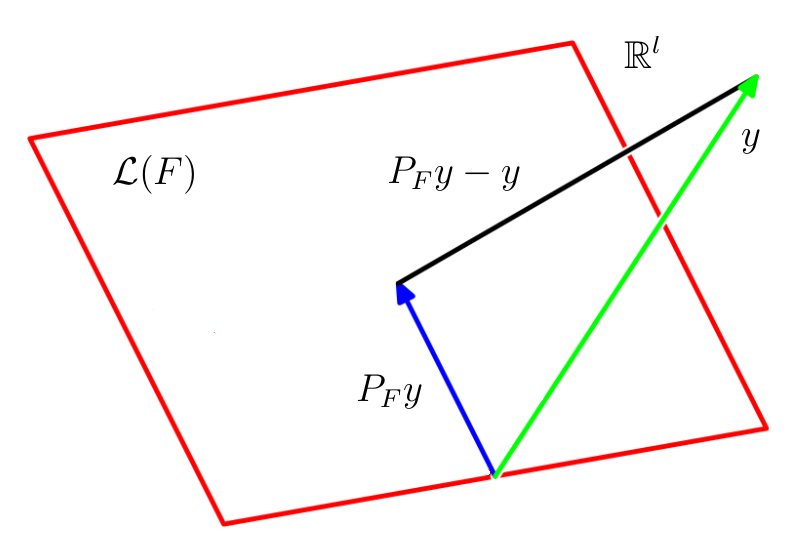
\includegraphics[height=200pt, keepaspectratio = true]{images/geometry}   
	\end{figure}
\end{frame}

{\foot{Singular value decomposition}
\begin{frame}{Сингулярное разложение}
	Произвольная $l \times n$-матрица представима в виде сингулярного разложения:\\
	$$X = VDU^T$$\\
	\bigbreak
	\pause
	Основные свойства сингулярного разложения:\\
	\begin{enumerate}[--]
		\item $V_{l \times n} = (v_1, \dots, v_n)$ ортогональна, $V^TV = I_n$, \\столбцы $v_j$ - собственные векторы матрицы $XX^T$
		\item $U_{n \times n} = (u_1, \dots, u_n)$ ортогональна, $U^TU = I_n$, \\столбцы $u_j$ - собственные векторы матрицы $X^TX$
		\item $D$ диагональна, $D_{n \times n} = \operatorname{diag} (\sqrt{\lambda_1}, \dots, \sqrt{\lambda_n})$, \\$\lambda_j > 0$ - собственные значения матриц $X^TX$ и $XX^T$
	\end{enumerate}
\end{frame}
}

\begin{frame}{Решение МНК через сингулярное разложение}
	Псевдообратная $X^+$, вектор МНК-решения $w^*$,
	МНК-аппроксимация целевого вектора $Xw^*$\\
	\bigbreak
	\pause
	$X^+ = (UDV^TVDU^T)^{-1}UDV^T = UD^{-1}V^T = \sum\limits_{j=1}^n \frac{1}{\sqrt{\lambda_j}}  u_j v_j^T$\\
	\pause
	$ w^* = X^+y = UD^{-1}V^Ty = \sum\limits_{j=1}^n \frac{1}{\sqrt{\lambda_j}}  u_j (v_j^Ty)$\\
	\pause
	$X w^* = P_X y = (VDU^T)UD^{-1}V^Ty = VV^Ty = \sum\limits_{j=1}^n v_j (v_j^Ty)$\\
	\pause
	$\Vert w^* \Vert^2  = \Vert D^{-1}V^Ty \Vert^2 = \sum\limits_{j=1}^n \frac{1}{\lambda_j} (v_j^Ty)^2$
\end{frame}

%\begin{frame}{Проблема мультиколлинеарности}
%	Если $\exists \gamma \in \mathbb{R}^n: X\gamma \approx 0$, то некоторые $\lambda_j$ близки к нулю.\\
%	\bigbreak
%	Число обусловленности $n \times n$-матрицы $X^TX = A$:
%	$$\mu(A) = \Vert A \Vert \Vert A^{-1} \Vert = \frac{\max\limits_{u: \Vert u \Vert = 1} \Vert A u \Vert}{\min\limits_{u: \Vert u \Vert = 1} \Vert A u \Vert} = \frac{\lambda_{max}}{\lambda_{min}}$$\\
%	\pause
%	При умножении обратной матрицы на вектор, $z = A^{-1}u$, относительная погрешность усиливается в $\mu(A)$ раз:\\
%	$$\frac{\Vert \delta z \Vert}{\Vert z \Vert } \leq \mu(A) \frac{\Vert \delta u \Vert}{\Vert u \Vert }$$
%\end{frame}

\begin{frame}{Проблема мультиколлинеарности}
	Если матрица $X^TX$ плохо обусловлена, то: 
	\begin{enumerate}[--]
		\item решение становится неустойчивым и неинтерпретируемым, $\Vert w^* \Vert $ велико
		\item $E_{in} = \Vert Xw^* -y \Vert$ -- мало   
		\item $E_{out} = \Vert X'w^* -y' \Vert$ -- велико
	\end{enumerate}
	\bigbreak
	\pause
	\alert{Вопрос:} Как бороться с этой проблемой?
\end{frame}

\begin{frame}{Проблема мультиколлинеарности}
	Стратегии устранения мультиколлинеарности и переобучения:
	\begin{enumerate}[--]
		\item Регуляризация: $\Vert w \Vert \rightarrow \min$
		\item Отбор признаков: $x^1, \dots, x^n \rightarrow x^{j_1}, \dots, x^{j_m}, \hspace{3mm} m << n$
		\item Преобразование признаков: $x^1, \dots, x^n \rightarrow g^1, \dots, g^m,\hspace{3mm}  m << n$
	\end{enumerate}
\end{frame}

{\foot{Ridge regression}
\begin{frame}{Гребневая регрессия}
	Штраф за увеличение нормы вектора весов $\Vert w \Vert$:\\
	$$Q_{\tau} (w) = \Vert X w - y \Vert^2 + \tau \Vert w \Vert^2$$\\
	где $\tau$ -- неотрицательный параметр регуляризации.\\
  \pause
	\bigbreak
	Модифицированное МНК-решение ($\tau I_n$ — «гребень»)\\
	$$w^*_{\tau} = (X^T X + \tau I_n)^{-1}X^Ty$$\\
  \pause	
  \bigbreak
	\alert{Вопрос:} Можно ли подбирать $\tau$ не вычисляя каждый раз обратную матрицу?
\end{frame}
}

\begin{frame}{Преимущество сингулярного разложения}
	Модифицированное МНК-решение ($\tau I_n$ — «гребень»)\\
	$$w^*_{\tau} = (X^TX + \tau I_n)^{-1}X^Ty$$\\
	\pause
	Преимущество сингулярного разложения:\\
	Можно подбирать параметр $\tau$ , вычислив сингулярное разложение только один раз.
\end{frame}

\begin{frame}{Сингулярное разложение}
	$$w_{\tau}^*= U(D^2 + \tau I_n)^{-1}DV^Ty = \sum\limits_{j=1}^n \frac{\sqrt{\lambda_j}}{\lambda_j + \textcolor{orange}{\tau}} u_j(v_j^Ty)$$\\
	\pause
	$$Xw_{\tau}^* = VDU^Tw_{\tau}^* = V \operatorname{diag} \left(\frac{\lambda_j}{\lambda_j + \tau}\right) V^Ty = \sum\limits_{j=1}^n \frac{\lambda_j}{\lambda_j + \textcolor{orange}{\tau}} v_j (v_j^Ty)$$\\
	\pause
	$$\Vert w_{\tau}^* \Vert^2 = \Vert (D^2 + \tau I_n)^{-1} DV^T y \Vert^2 = \sum\limits_{j=1}^n \frac{\lambda_j}{(\lambda_j + \textcolor{orange}{\tau})^2} (v^T_j y)^2$$\\
	\pause
	$X w_{\tau}^* \neq Xw^*$ -- зато решение становится более устойчивым
\end{frame}

\begin{frame}{Выбор параметра регуляризации $\tau$}
	Контрольная выборка: $X^k = (x'_i, y'_i)_{i=1}^k$\\
	%Вычисление функционала $Q$ на контрольных данных $T$ раз потребует $O(kn^2 + knT)$ операций:\\
	$$Q(w_{\tau}^*,X^k) = \Vert X' w_{\tau}^* - y' \Vert^2 = \Vert X'U \operatorname{diag} \left(\frac{\lambda_j}{\lambda_j + \tau}\right) V^T y -y' \Vert^2$$\\
	\bigbreak
	\pause
	Зависимость $Q(\tau)$ обычно имеет характерный минимум.
\end{frame}

%\begin{frame}{Сокращение «эффективной размерности»}
%	Сокращение весов:\\
%	$$\Vert w_{\tau}^* \Vert^2 = \sum\limits_{j=1}^n \frac{\lambda_j}{(\lambda_j + \tau)^2} (v^T_j y)^2 < \Vert w^* \Vert^2  = \sum\limits_{j=1}^n \frac{1}{\lambda_j} (v_j^Ty)^2$$\\
%	\pause
%	Роль размерности играет след проекционной матрицы:\\
%	$$tr X(X^TX)^{-1}X^T = tr(X^TX)^{-1}X^TX = tr I_n = n$$
%  \bigbreak	
%	\pause
%	При использовании регуляризации:\\
%	$$tr X(X^TX + \tau I_n)^{-1}X^T = tr \hspace{1mm}  \operatorname{diag} \left(\frac{\lambda_j}{\lambda_j + \tau}\right)= \sum\limits_{j=1}^n \frac{\lambda_j}{\lambda_j + \tau } < n $$
%\end{frame}

{\foot{LASSO, Least Absolute Shrinkage and Selection Operator}
\begin{frame}{Лассо Тибширани}
	$$
	\begin{cases} Q(w,X^l) = \Vert Xw - y \Vert^2 \rightarrow \min\limits_{w} \\
	\sum_{j=1}^n \vert w_j \vert \leq \kappa
	\end{cases}
	$$\\
	\pause
	После замены переменных:\\
	$$
	\begin{cases} w_j = w_j^+ - w_j^-\\
	\vert w_j \vert = w_j^+ + w_j^-, \hspace{5mm} w_j^+, w_j^- \geq 0\\
	
	\end{cases}
	$$\\
	ограничения принимают канонический вид:\\
	$$\sum\limits_{j=1}^n w_j^+ + w_j^- \leq \kappa$$\\
	\pause
	Чем меньше $\kappa$, тем больше $j$ таких, что $w_j^+ = w_j^- = 0$\\
	%не гауссовское распределение, а лапласовское
\end{frame}
}

%\begin{frame}{Негладкие регуляризаторы}
%	Elastic Net:\\
%	$$\frac{1}{2} \Vert Xw - y \Vert^2 + \mu \sum\limits_{j=1}^n \vert w_j \vert + \frac{\tau}{2} \sum\limits_{j=1}^n w_j^2 \rightarrow \min\limits_{w}$$\\
%	\pause
%	Support Features Machine:\\
%	$$\frac{1}{2} \Vert Xw - y \Vert^2 + \tau \sum\limits_{j=1}^n R_{\mu}(w_j) \rightarrow \min\limits_{w}$$\\
%	$$ R_{\mu}(w_j) = \begin{cases} 2 \mu \vert w_j \vert, \hspace{2mm} \vert w_j \vert \leq \mu\\
%	\mu^2 + w_j^2, \hspace{2mm} \vert w_j \vert \geq \mu
%	\end{cases}$$\\
%\end{frame}

\section{Нелинейная регрессия}

\begin{frame}{Нелинейная регрессия}
	\alert{Вопрос:} Что изменится, если модель регрессии не линейна?\\
	\bigbreak
	$$f(x, w), \hspace{5mm} w \in \mathbb{R}^p$$
\end{frame}

\begin{frame}{Метод Ньютона-Рафсена}
	Начальное приближение $w^{(0)} = (w_1^{(0)}, \dots, w_p^{(0)})$\\
	Итерационный процесс: $w^{(t+1)} = w^{(t)} - h_t (Q''(w^{(t)}))^{-1}Q'(w^{(t)})$\\
	\bigbreak
	$Q'(w^{(t)})$ -- градиент функционала $Q$ в точке $w^{(t)}$\\
	$Q''(w^{(t)})$ -- гессиан функционала $Q$ в точке $w^{(t)}$\\
	$h_t$ -- величина шага
\end{frame}

\begin{frame}{Метод Ньютона-Рафсена}
	$$Q(w,X^l) = \sum\limits_{i=1}^l (f (x_i, w) - y_i)^2 \rightarrow \min\limits_{w}$$\\
	
	$$\frac{\partial Q(w)}{\partial w_j} = 2 \sum\limits_{i=1}^l (f(x_i, w) - y_i ) \frac{\partial(f(x_i, w))}{\partial w_j}$$\\
	$$\frac{\partial^2 Q(w)}{\partial w_j \partial w_k} = 2 \sum\limits_{i=1}^l \frac{\partial(f(x_i, w))}{\partial w_j} \frac{\partial(f(x_i, w))}{\partial w_k} - 2 \sum\limits_{i=1}^l (f(x_i, w) - y_i ) \frac{\partial^2 (f(x_i, w))}{\partial w_j \partial w_k}$$\\
	\bigbreak
	\pause
	\alert{Вопрос:} Какая часть самая тяжелая?
\end{frame}

\begin{frame}{Метод Ньютона-Рафсена}
	$$\frac{\partial Q(w)}{\partial w_j} = 2 \sum\limits_{i=1}^l (f(x_i, w) - y_i ) \frac{\partial(f(x_i, w))}{\partial w_j}$$\\
	$$\frac{\partial^2 Q(w)}{\partial w_j \partial w_k} = 2 \sum\limits_{i=1}^l \frac{\partial(f(x_i, w))}{\partial w_j} \frac{\partial(f(x_i, w))}{\partial w_k} - 2 \sum\limits_{i=1}^l (f(x_i, w) - y_i ) \frac{\partial^2 (f(x_i, w))}{\partial w_j \partial w_k}$$\\
	\bigbreak
	\pause
	Линеаризация $f(x_i, w)$ в окрестности текущего $w^{(t)}$:\\
	$$f(x_i, w) = f(x_i, w^{(t)}) + \sum\limits_{j=1}^p \frac{\partial(f(x_i, w))}{\partial w_j} (w_j - w_j^{(t)}) + o(w_j -w_j^{(t)})$$\\
	$\Rightarrow$ второе слагаемое в гессиане обнулилось
\end{frame}

\begin{frame}{Матричные обозначения}
	$X_t = \left(\frac{\partial(f(x_i, w^{(t)}))}{\partial w_j^{(t)}}\right)_{l \times p}$ -- матрица первых производных\\
	$f_t = \left( f(x_i, w^{(t)}) \right)_{l \times 1}$ -- вектор значений $f$\\
	\bigbreak
	Формула $t$-й итерации метода Ньютона–Гаусса:\\
	$$w^{(t+1)} = w^{(t)} - h_t \underbrace{\left( X^T_t X_t \right)^{-1} X_t^T(f_t -y)}_{\beta}$$\\
	где $\beta$ -- решение многомерной линейной регрессии\\
	$$\Vert X_t\beta - (f_t-y) \Vert^2 \rightarrow \min_{\beta}$$ 
\end{frame}

\begin{frame}{Метод Ньютона-Рафсена}
	\begin{figure}[htbp]
	  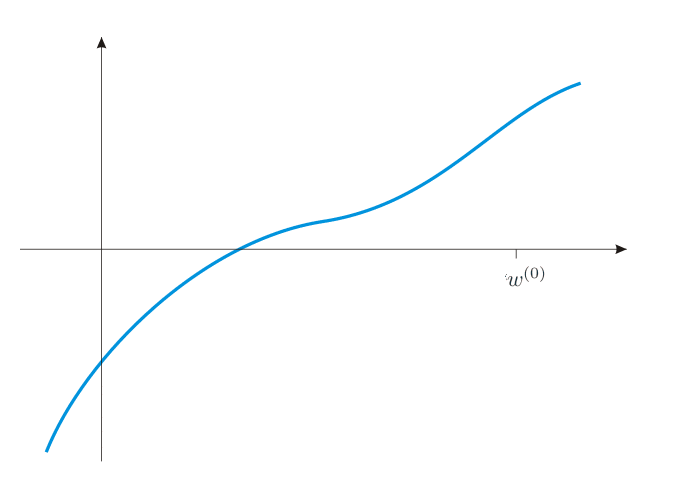
\includegraphics[height=150pt, keepaspectratio = true]{images/newton-1}   
	\end{figure}
\end{frame}

\begin{frame}{Метод Ньютона-Рафсена}
	\begin{figure}[htbp]
	  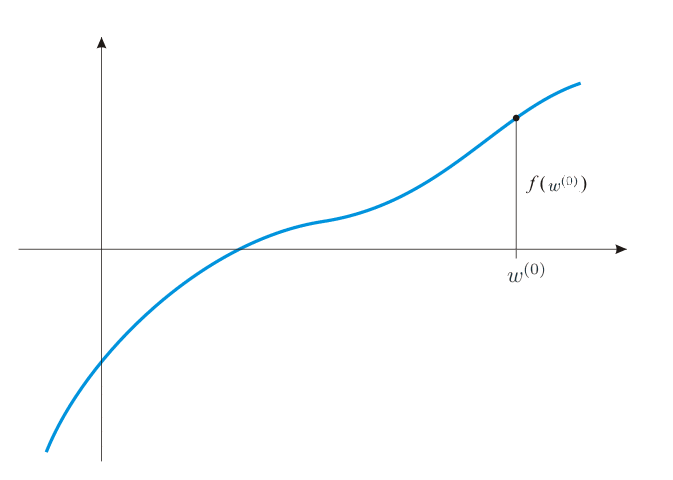
\includegraphics[height=150pt, keepaspectratio = true]{images/newton-2}   
	\end{figure}
\end{frame}

\begin{frame}{Метод Ньютона-Рафсена}
	\begin{figure}[htbp]
	  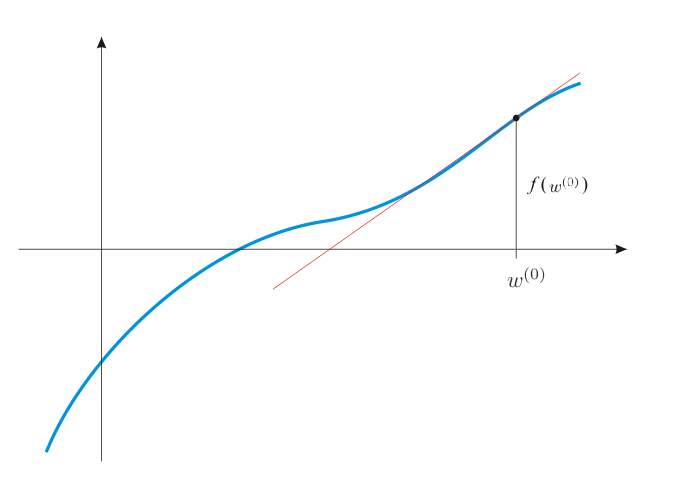
\includegraphics[height=150pt, keepaspectratio = true]{images/newton-3}   
	\end{figure}
\end{frame}

\begin{frame}{Метод Ньютона-Рафсена}
	\begin{figure}[htbp]
	  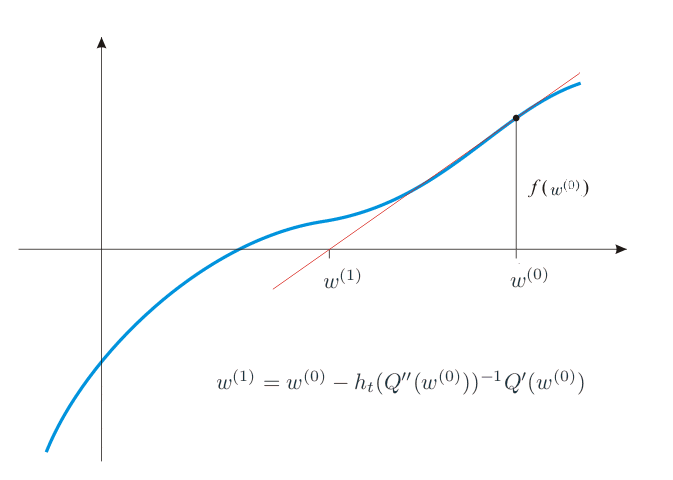
\includegraphics[height=150pt, keepaspectratio = true]{images/newton-4}   
	\end{figure}
\end{frame}

\begin{frame}{Метод Ньютона-Рафсена}
	\begin{figure}[htbp]
	  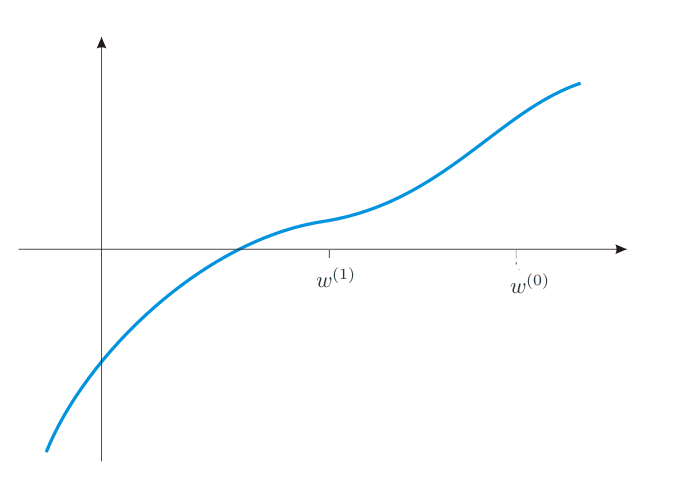
\includegraphics[height=150pt, keepaspectratio = true]{images/newton-5}   
	\end{figure}
\end{frame}

\begin{frame}{Метод Ньютона-Рафсена}
	\begin{figure}[htbp]
	  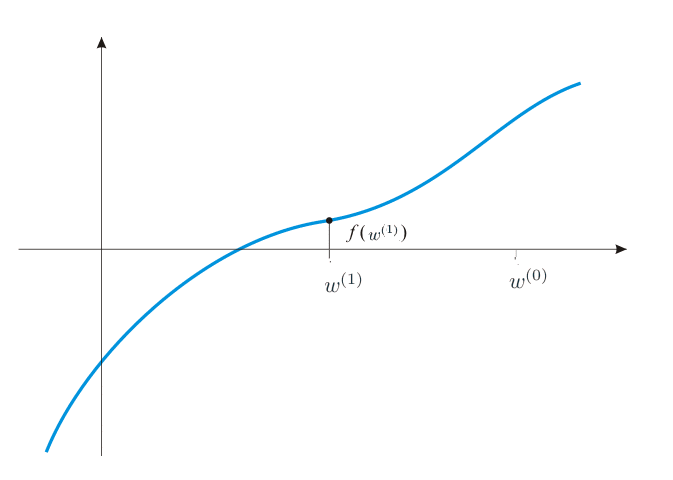
\includegraphics[height=150pt, keepaspectratio = true]{images/newton-6}   
	\end{figure}
\end{frame}

\begin{frame}{Метод Ньютона-Рафсена}
	\begin{figure}[htbp]
	  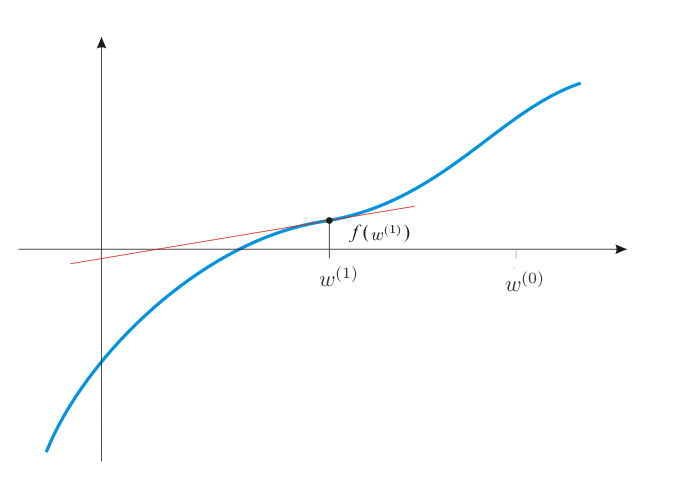
\includegraphics[height=150pt, keepaspectratio = true]{images/newton-7}   
	\end{figure}
\end{frame}

\begin{frame}{Метод Ньютона-Рафсена}
	\begin{figure}[htbp]
	  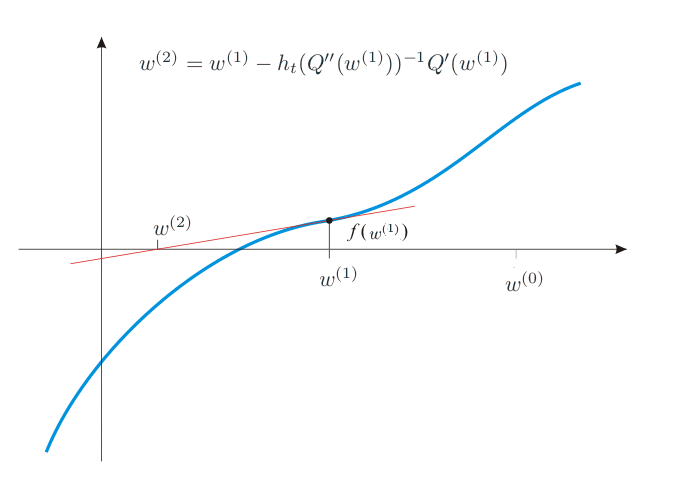
\includegraphics[height=150pt, keepaspectratio = true]{images/newton-8}   
	\end{figure}
\end{frame}

\begin{frame}{Метод Ньютона-Рафсена}
	\begin{figure}[htbp]
	  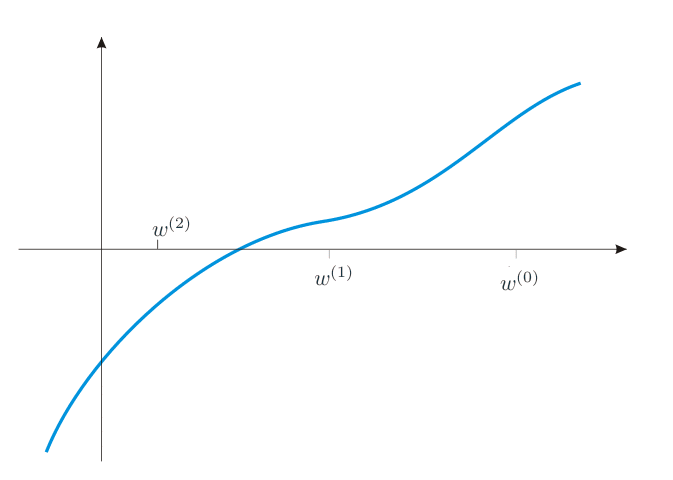
\includegraphics[height=150pt, keepaspectratio = true]{images/newton-9}   
	\end{figure}
\end{frame}

\begin{frame}{Метод Ньютона-Рафсена}
	\begin{figure}[htbp]
	  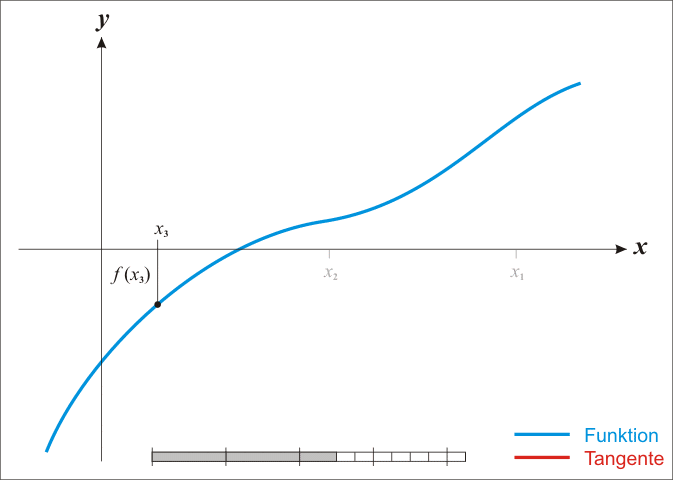
\includegraphics[height=150pt, keepaspectratio = true]{images/newton-10}   
	\end{figure}
\end{frame}

\begin{frame}{Метод Ньютона-Рафсена}
	\begin{figure}[htbp]
	  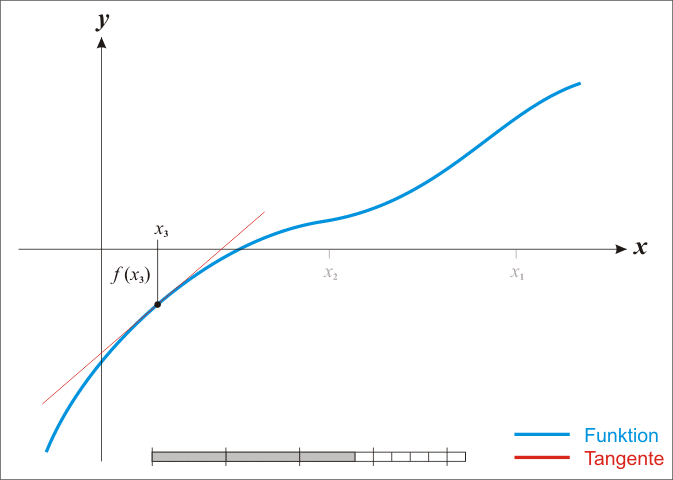
\includegraphics[height=150pt, keepaspectratio = true]{images/newton-11}   
	\end{figure}
\end{frame}

\begin{frame}{Метод Ньютона-Рафсена}
	\begin{figure}[htbp]
	  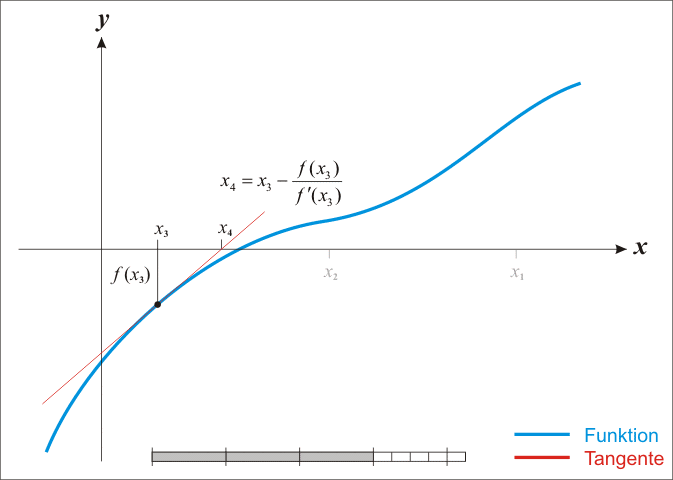
\includegraphics[height=150pt, keepaspectratio = true]{images/newton-12}   
	\end{figure}
\end{frame}

\begin{frame}{Метод Ньютона-Рафсена}
	\begin{figure}[htbp]
	  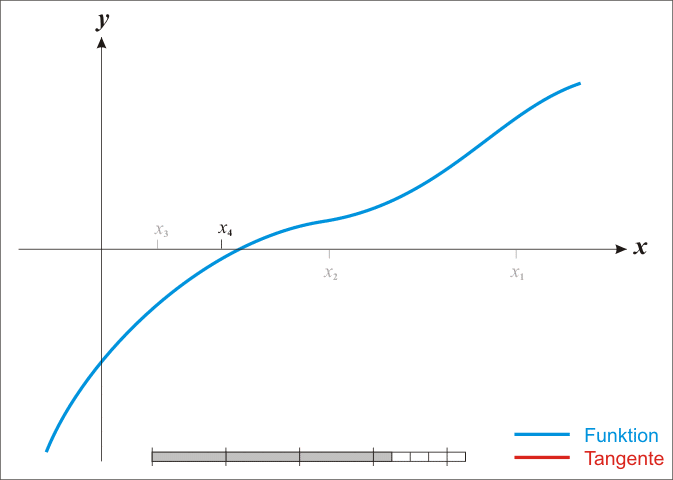
\includegraphics[height=150pt, keepaspectratio = true]{images/newton-13}   
	\end{figure}
\end{frame}

\begin{frame}{Метод Ньютона-Рафсена}
	\begin{figure}[htbp]
	  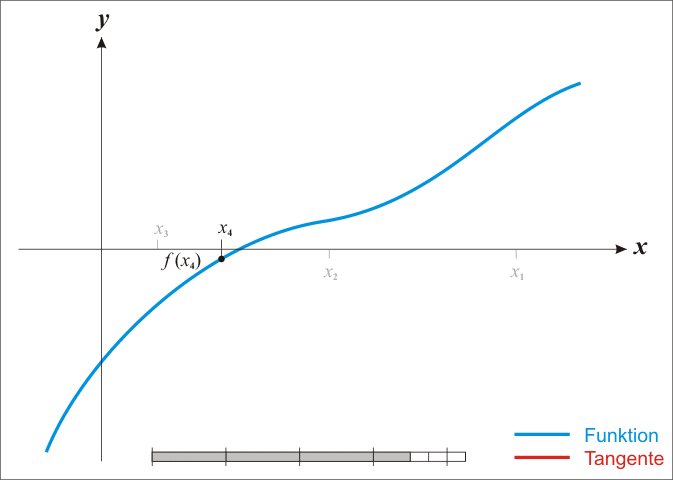
\includegraphics[height=150pt, keepaspectratio = true]{images/newton-14}   
	\end{figure}
\end{frame}

\begin{frame}{Метод Ньютона-Рафсена}
	\begin{figure}[htbp]
	  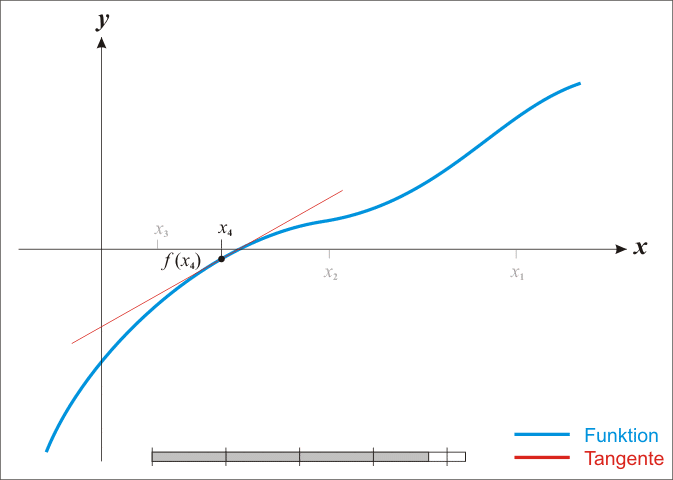
\includegraphics[height=150pt, keepaspectratio = true]{images/newton-15}   
	\end{figure}
\end{frame}

\begin{frame}{Метод Ньютона-Рафсена}
	\begin{figure}[htbp]
	  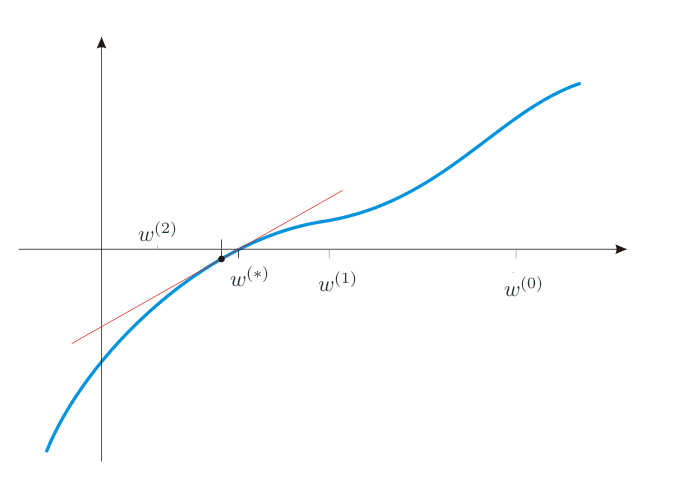
\includegraphics[height=150pt, keepaspectratio = true]{images/newton-16}   
	\end{figure}
\end{frame}

\begin{frame}{Метод Ньютона-Рафсена}
	\begin{figure}[htbp]
	  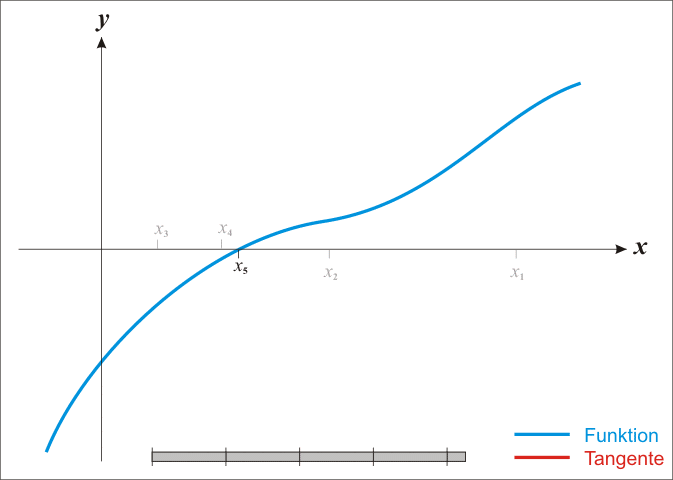
\includegraphics[height=150pt, keepaspectratio = true]{images/newton-17}   
	\end{figure}
\end{frame}

\begin{frame}[standout]
  Вопросы?
\end{frame}

\appendix

\section{Метод главных компонент}

\begin{frame}{Метод главных компонент}
	$x^1, \dots, x^n$ -- исходные числовые признаки\\
	$g^1(x), \dots, g^m(x)$ -- новые числовые признаки, $m \times n$\\
	\bigbreak
	\textbf{Вопрос:} Как сформулировать требование к новым признакам?
\end{frame}

\begin{frame}{Метод главных компонент}
	$x^1, \dots, x^n$ -- исходные числовые признаки\\
	$g_1(x), \dots, g_m(x)$ -- новые числовые признаки, $m \times n$\\
	\bigbreak
	\pause
	Требование: старые признаки должны линейно восстанавливаться по новым:\\
	$$\hat{f}_j(x) = \sum\limits_{s=1}^m g_s(x) u_{js} , \hspace{2mm} j = 1,\dots , n, \hspace{2mm} \forall x \in X$$\\
	как можно точнее на обучающей выборке $x_1, \dots, x_l$:\\
	$$\sum\limits_{i=1}^l \sum\limits_{j=1}^n (\hat{f}_j(x_i) - f_j(x_i))^2 \rightarrow \min\limits_{g_s(x_i), u_{js}}$$
\end{frame}

\begin{frame}{Матричные обозначения}
	$$\underset{l \times n}{X} = \begin{pmatrix}
	  f_1(x_1) & \dots & f_n(x_1) \\
	  \dots & \dots & \dots\\
	  f_1(x_l) & \dots & f_n(x_l)
	 \end{pmatrix} \hspace{1mm} 
	 \underset{l \times m}{G} = \begin{pmatrix}
	  g_1(x_1) & \dots & g_m(x_1) \\
	  \dots & \dots & \dots\\
	  g_1(x_l) & \dots & g_m(x_l)
	 \end{pmatrix}$$\\
	 $$\underset{n \times m}{U} = \begin{pmatrix}
	  u_{11} & \dots & u_{1m} \\
	  \dots & \dots & \dots\\
	  u_{n1} & \dots & u_{nm}
	 \end{pmatrix}$$
	$U$ -- линейное преобразование новых признаков в старые\\
	$$\hat{X} = GU^T \approx X$$\\
	\pause
	\alert{Найти:} новые признаки $G$ и преобразование $U$:\\
	$$\sum\limits_{i=1}^l \sum\limits_{j=1}^n (\hat{x}_i^j - x_i^j)^2 = \Vert GU^T - X \Vert^2 \rightarrow \min\limits_{G, U}$$
\end{frame}

\begin{frame}{Основная теорема}
	Если $m < \rank X$, то минимум $\Vert GU^T - X \Vert^2$ достигается, когда столбцы $U$ - это с.в. матрицы $X^TX$, соответствующие $m$ максимальным с.з. $\lambda_1,\dots, \lambda_m$, а матрица $G = XU$.\\
	\bigbreak
	\pause
	При этом:\\
	\begin{itemize}
		\item матрица $U$ ортонормирована: $U^TU = I_m$
		\item матрица $G$ ортогональна: $G^TG = \Lambda = \operatorname{diag}(\lambda_1, \dots, \lambda_m)$
		\item $U\Lambda = X^TXU$,  $G\Lambda = FF^TG$
		\item $\Vert GU^T - X \Vert^2 = \Vert X \Vert^2 - tr \Lambda = \sum\limits_{j=m+1}^n \lambda_j$
	\end{itemize}
\end{frame}

\begin{frame}{Связь с сингулярным разложением}
	Если взять $m = n$, то:\\
	\begin{itemize}[<+->]
	\item $\Vert GU^T - X \Vert^2 = 0$
	\item представление $\hat{X} = GU^T = X$ точное и совпадает с сингулярным разложением при $G = V \sqrt{\Lambda}$
	$$X = GU^T = V\sqrt{\Lambda}U^T, \hspace{2mm} U^TU = I_m, \hspace{2mm} V^TV = I_m$$
	\item линейное преобразование $U$ работает в обе стороны:\\
	$$X = GU^T, \hspace{4mm} G=XU$$
	Преобразование $U$ называется декоррелирующим
	\end{itemize}
\end{frame}

\begin{frame}{Эффективная размерность выборки}
	Упорядочим с.з. $X^TX$ по убыванию: $\lambda_1 > \dots > \lambda_n > 0$\\
	Эффективная размерность выборки -- это наименьшее целое $m$, при котором\\
	$$E_m = \frac{\Vert GU^T - X \Vert^2}{\Vert X \Vert^2} = \frac{\lambda_{m+1} + \dots + \lambda_{n}}{\lambda_1 + \dots + \lambda_n} \leq \varepsilon$$\\
	\pause
	Критерий «крутого склона»: находим $m: E_{m-1} >> E_m$:
	\begin{figure}[htbp]
	  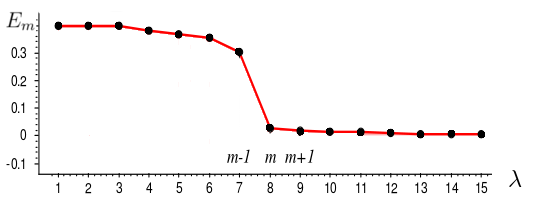
\includegraphics[height=100pt, keepaspectratio = true]{images/edge}   
	\end{figure}
\end{frame}

\begin{frame}{Решение задачи НК в новых признаках}
	Заменим $F$ на её приближение $GU^T$:\\
	$$\Vert GU^Tw -y \Vert^2 = \Vert G\hat{w} -y \Vert^2 \rightarrow \min\limits_{\hat{w}}$$\\
	Связь нового и старого вектора коэффициентов:\\
	$$w = U\hat{w}, \hspace{5mm} \hat{w} = U^T w$$\\
	\pause
	\bigbreak
	Решение задачи наименьших квадратов относительно $\hat{w}$ (единственное отличие -- $m$ слагаемых вместо $n$):\\
	$$\hat{w}^* = D^{-1}V^Ty = \sum\limits_{j=1}^m \frac{1}{\sqrt{\lambda_j}} u_j (v_j^Ty)$$\\
	$$G\hat{w}^* = VV^Ty = \sum\limits_{j=1}^m v_j (v_j^Ty)$$
\end{frame}

\begin{frame}{На следующей лекции}
	\begin{itemize}
    	\item[--] Bias-variance tradeoff
    	\item[--] Кривые обучения 
	\end{itemize}
\end{frame}

\end{document}
